\documentclass{article}[11pt]
\usepackage{arxiv}
\usepackage{url}

\usepackage{amssymb, amsmath}
\usepackage{amsthm}
\newtheorem{lemma}{Lemma}
\newtheorem{theorem}{Theorem}
\newtheorem{proposition}{Proposition}

\usepackage{algorithm}
\usepackage{algpseudocode}

\setlength{\jot}{12pt}

\usepackage{graphicx}
\graphicspath{{fig/}}
\usepackage[export]{adjustbox}

\begin{document}
	
	
	\title{Neural Networks for Classification}
	\author{Owen Jones (olj23\@bath.ac.uk)}
	\date{Spring 2019}
	\maketitle


\begin{abstract}
    
    %TODO
    
	Here is the contents of my abstract blah blah blah blah blah.
\end{abstract}



\section{Introduction to Classification Problems}

    
    
    
    
    
    
    
    
    
    
    
    
    Historically, machine learning tasks have fallen into one of several categories: supervised learning problems, unsupervised learning problems, and more recently reinforcement learning
    
    Classification tasks (in the sense which this paper considers) belong to the supervised learning family of tasks, where the data used in the training process is \textit{labelled}
    
    qualitative outputs
    
    In Section \ref{sec:demos} of this paper, the 



\section{Logistic Regression} \label{sec:logreg}

    Consider any question where the answer is either "yes" or "no". Will the next train arrive on time? Does this image contain a face? Should we prescribe this patient Drug B instead of Drug A? In this way, many problems in the real world can be reduced in essence to a \textit{binary classification} task, where the "correct" answer belongs to one of two distinct categories.

    Therefore if we wish to produce a model capable of performing classification tasks, a useful starting point would be a binary classifier: that is, we would like to produce a model $f$ which, given some observation $\mathbf{x}$ with an associated label $y \in \{0, \ 1\}$, produces a result such that
    
    $$
    f(\mathbf{x}) \approx y \,.
    $$
    
    This section outlines the motivation behind and the definition of one of the best-known binary classifiers, the \textit{logistic regression} model.



    \subsection{Linear Regression}
        
        A reasonable assumption when beginning to define a model is that the class of the observation is somehow related to its features - if that is not the case, then we will struggle to extract any meaningful information from the data available to us!
        
        Therefore suppose we have an observation $\mathbf{x}$ consisting of $n \geq 1$ inputs:
        
        $$
        \mathbf{x} = (x_1, \ x_2, \ \ldots, \ x_{n-1}, \ x_n) \in \mathbb{R}^n \,.
        $$
        
        Let us define a set of weights $\boldsymbol{\theta} = (\theta_0, \ldots, \theta_n) \in \mathbb{R}^{n+1}$ which in combination with $\mathbf{x}$ produce a scalar output
        
        $$
        z = \theta_0 + \sum_{k=1}^n \theta_k x_k \,.
        $$
        
        Notice the additional \textit{bias} weight $\theta_0$, which corresponds to a shift in the output independent of any of the inputs. To simplify notation later on, we can redefine $\mathbf{x} \in \mathbb{R}^{n+1}$ by augmenting with $x_0 = 1$, which allows us to write $z$ as a single summation:
        
        $$
        z = \sum_{k=0}^n \theta_k x_k = \boldsymbol{\theta}^\top \mathbf{x} \,.
        $$
        
        By adjusting the weights $\theta_0, \ldots, \theta_n$, the same inputs $\mathbf{x}$ can give us a completely different output. Note that if we do not restrict $\boldsymbol{\theta}$ then $z$ is unbounded, i.e. $z \in (-\infty, \infty)$.
        
        
        
    \subsection{Introducing Non-Linearity}
        
        Recall that the goal of a binary classification task is to assign a categorical label to each observation; so if we wish to use linear regression as the basis for our algorithm, ultimately we will need to somehow interpret the continuous output $z \in \mathbb{R}$ as corresponding to one of those discrete labels.
        
        This can be achieved by means of a non-linear \textit{activation function}:
        
        $$
        \sigma \colon (-\infty, \infty) \to (0, 1) \,.
        $$
        
        In later sections we will consider other activation functions, but for logistic regression we typically use the \textit{sigmoid} function,
            
        $$
        \sigma_2(z) = \frac{1}{1 + e^{-z}} \,.
        $$
        
        
        % TODO sigmoid plot
        
        
        Note how large positive values of $z$ are approximately mapped to 1, large negative values are approximately mapped to 0, and the transition between the two asymptotic limits is relatively sudden, yet smooth, with the central "threshold" at $z = 0$.
        
        In the remainder of this paper, the activated output $\sigma(z)$ is sometimes denoted as $a$ for the sake of notational simplicity.
        
        
        
    \subsection{Quantifying Incorrectness} \label{sec:costfun}
        
        Now that we have a means of mapping an input $\mathbf{x}$ to an activated output $a \in (0, 1)$, we can begin to think about how to adjust the weights $\boldsymbol{\theta}$ so that $a$ is as close to the target output $y$ as possible.
        
        In order to assess how well the model is performing, we shall require some sort of "penalty value" based on the dissimilarity between $a$ and $y$. For example, the \textit{binary cross-entropy} is defined as follows:
        
        $$
        CE(a, y \ \vert \ \boldsymbol{\theta}) = \begin{cases}
            -\log(a) & y = 1 \\
            -\log(1-a) & y = 0
        \end{cases} \,.
        $$
        
        
        % TODO plot
        
        
        Note that $CE$ is a function of $\boldsymbol{\theta}$ (since $a$ is a function of $z$, which is dependent on $\boldsymbol{\theta}$), that it takes a value of 0 if $a = y$, and that it increases exponentially as $a$ becomes further from $y$.
        
        So far we have considered a single observation $\mathbf{x}$ with a label $y$, which in combination with $\boldsymbol{\theta}$ produces a single activated output $a$. However in reality, we have multiple observations (say $m \geq 1$) each with an associated label and each producing an activated output in combination with $\boldsymbol{\theta}$. Therefore when assessing how well $\boldsymbol{\theta}$ parameterises our entire set of observations, we need to consider the cost of each of those observations.
        
        For that purpose, we generally consider some \textit{cost function} $J(\boldsymbol{\theta})$ which combines the individual costs from each observation. Such a function effectively quantifies how "wrong" the model is, so when adjusting $\boldsymbol{\theta}$ we will be aiming to minimise $J(\boldsymbol{\theta})$. A typical choice for binary classification problems is the \textit{binary cross-entropy cost function}:
        
        $$
        J_2(\boldsymbol{\theta}) = \frac{1}{m} \sum_{i=1}^{m} CE(\boldsymbol{\theta}) = - \frac{1}{m} \sum_{i=1}^{m} \left( y_i \log(a_i) + (1 - y_i) \log(1 - a_i) \right) \,.
        $$
        
        Since $y_i \in \{0, 1\}$, at most one of the terms in the body of the summation is non-zero for each $i$; and so $J_2(\boldsymbol{\theta})$ is simply the average cross-entropy across all $m$ observations in our dataset.
    
    

    \subsection{Training} \label{sec:gradient_descent}
        
        As described at the end of Section \ref{sec:costfun}, the goal of the \textit{training} process is to minimise the cost function $J(\boldsymbol{\theta})$ by making changes to the parameters $\boldsymbol{\theta}$: in other words, we essentially have an optimisation problem, which we can tackle in countless different ways.
        
        Here we will focus on \textit{gradient descent}, an iterative method which takes successive steps converging towards a minimum optimal value. Although many other more sophisticated optimisation algorithms exist, gradient descent is one of the most commonly used optimisation methods due to its simplicity yet relative effectiveness: see \cite{lecun_backprop} for further details.
        
        
        
        \subsubsection{Descent Direction}
            
            Since we wish to reduce $J(\boldsymbol{\theta})$ by taking some step in parameter space, before doing anything else we must determine the direction in which to take that step.
            
            Consider a perturbation $\Delta \boldsymbol{\theta}$ to our current parameters $\boldsymbol{\theta} \in \mathbb{R}^{n+1}$, and notice that a Taylor expansion yields
            
            $$
            J(\boldsymbol{\theta} + \Delta \boldsymbol{\theta}) = J(\boldsymbol{\theta}) + \sum_{k=0}^{n+1} \frac{\partial J(\boldsymbol{\theta})}{\partial \theta_k} (\Delta \boldsymbol{\theta})_k + \mathcal{O} ((\Delta \boldsymbol{\theta})^2) \,.
            $$
            
            Then ignoring higher-order terms, we have
            
            $$
            J(\boldsymbol{\theta} + \Delta \boldsymbol{\theta}) \approx J(\boldsymbol{\theta}) + \nabla J(\boldsymbol{\theta})^\top \Delta \boldsymbol{\theta} \,.
            $$
            
            Now we greedily choose $\Delta \boldsymbol{\theta}$ such that we reduce $J(\boldsymbol{\theta})$ by as much as possible - i.e. by making $\nabla J(\boldsymbol{\theta})^\top \Delta \boldsymbol{\theta}$ as negative as possible. By the Cauchy-Schwarz inequality, the most negative value of $\mathbf{f}^\top \mathbf{g}$ for any $\mathbf{f}, \mathbf{g} \in \mathbb{R}^{n+1}$ is $- \lVert \mathbf{f} \rVert_2 \lVert \mathbf{g} \rVert_2$, when $\mathbf{f} = -\mathbf{g}$. Therefore we shall choose $\Delta \boldsymbol{\theta} = - \nabla J(\boldsymbol{\theta})$ as our \textit{descent direction}. Note that $\nabla J(\boldsymbol{\theta})^\top (- \nabla J(\boldsymbol{\theta})) = -\lVert \nabla J(\boldsymbol{\theta}) \rVert_2^2 \leq 0$ with equality if and only if $\nabla J(\boldsymbol{\theta}) = 0$, and consequently $J(\boldsymbol{\theta} + \Delta \boldsymbol{\theta}) < J(\boldsymbol{\theta})$ so long as $\nabla J(\boldsymbol{\theta}) \neq 0$.
        
    
    
        \subsubsection{Learning rate}
            
            While it is guaranteed that the "steepest descent" direction we have just chosen, $\Delta \boldsymbol{\theta} = - \nabla J(\boldsymbol{\theta})$, is indeed a descent direction, we must recall at this point that we are using a Taylor series approximation for $J(\boldsymbol{\theta} + \Delta \boldsymbol{\theta})$. Therefore this guarantee only applies in some (potentially very small) radius of the parameter space, centred on $\boldsymbol{\theta}$.
            
            Consequently in order to ensure that we obtain a reduction in $J$, we must scale $\Delta \boldsymbol{\theta}$ by some value $\eta$. This value is called the \textit{learning rate}.
            
            Selecting a learning rate is often a delicate task. Too small a value results in undersized steps in the descent direction, meaning convergence might be slow; too large a value may result in "overshooting" the region where descent is guaranteed, leading to oscillation around the optimum or even to complete divergence.
            
            As such, it is often favourable to use an \textit{adaptive learning rate}: rather than a fixed constant $\eta$, a new value $\eta_k$ is used at each iteration of the algorithm. Many methods exist for determining such adaptive rates, often based on line search methods - see \cite{line_search} and \cite{adam}.
            
            In this paper we will use a relatively simple method based on backtracking line search, where the learning rate is steadily grown by some constant factor at each iteration, and then more dramatically decreased when it is too large.
            
            
            \begin{algorithm} \label{alg:grow_and_slash}
                
                \caption{"Grow and slash" learning rate}
                
                \begin{algorithmic}
                
                    \State Choose $\eta_1 > 0$, $\alpha > 1$, $\beta > 1$ (in practice, $\alpha = 1.1$, $\beta = 2$ work well).
                    
                    \For {iterations $k = 1, ...$ of gradient descent}
                        \While {$J(\boldsymbol{\theta} + \eta_k (\Delta \boldsymbol{\theta})) > J(\boldsymbol{\theta})$}
                            \State $\eta_k \gets \eta_k / \beta$
                        \EndWhile
                        
                        \State $\eta_{k+1} \gets \alpha \eta_k$
                    \EndFor
                    
                \end{algorithmic}
            
            \end{algorithm}
            
            
    
    \subsection{Assessing Performance}
        
        When developing a model, it is essential to know how well the model is performing - both in terms of relating the output back to the original input data, and for the purpose of comparing the performance different models. This implies that we will require at least one \textit{performance metric}, which somehow quantifies how well the model is completing the task at hand.
        
        Arguably the simplest such metric is \textit{accuracy}, i.e. the proportion of observations which the network predicts correctly as belonging to their associated class. Accuracy is measured on a scale of 0 to 1, where 0 corresponds to a model which predicts everything incorrectly and 1 corresponds to every observation being classified correctly.
        
        The problems we will consider in Section \ref{sec:demos} of this paper will use data with \textit{balanced classes}, where an identical (or very similar) proportion of the data belongs to each class. This means it is reasonable for us to use accuracy as our performance metric, since poor performance on any class will affect the overall accuracy evenly.
        
        Consider, however, a case of imbalanced classes - say 90\% of observations belonging to one, and 10\% to another. A model which simply predicts that every observation belongs to the first class would achieve 90\% accuracy without serving any useful purpose at all! Therefore many other performance metrics have been developed (perhaps most famously, \textit{precision}, \textit{recall} and \textit{$F_1$ score}) which penalise mistakes differently, depending on their perceived significance.
        


\section{Neural Networks}
    
    The logistic regression model is, by definition, a \textit{linear classifier}: the output is directly linked (via the sigmoid function) to the weighted sum of the inputs. Since we are using such a model for binary classification, we set some threshold (generally 0.5 for sigmoid) such that all outputs above the threshold are mapped to one class, and all outputs below are mapped to the other. We can thus think of the decision boundary as a hyperplane which divides the problem's feature space into two halves.
    
    However, such a linear boundary may not be particularly suitable - the classes may not be linearly separable, meaning we could never achieve perfect accuracy with our model. Moreover we are only able to distinguish between binary-labelled data, which is not particularly useful if our observations can belong to more than two classes.
    
    Hence we would like to extend our logistic regression model, to allow for an arbitrary number of outputs to be predicted and for the construction of potentially non-linear decision boundaries.
    
    

    \subsection{Multiple Outputs} \label{sec:multi_out}
    
        So far we have considered passing the input $\mathbf{x}$ into a single logistic regression model, yielding a single scalar output $a$.
    
        By passing the same input $\mathbf{x}$ to $n$ separate logistic regression models, we can obtain $n$ separate outputs $a_1, \ldots, a_n$. If each model is initialised with a different set of weights $\boldsymbol{\theta_n}$, each would produce a slightly different output.
        
        Now suppose that we have a classification problem where each observation can belong to one of $n \geq 2$ classes. We can characterise the target output as a \textit{one-hot encoded} vector $\mathbf{y} \in \mathbb{R}^n$: for $\mathbf{x}$ belonging to class $k$, we define
        
        $$
        y_k = \begin{cases}
            1 & \text{observation belongs to class } k \\
            0 & \text{otherwise}
        \end{cases} \,.
        $$
        
        Thus we can train the $k$th model to produce an output of 1, and the other $(n-1)$ models to produce an output of 0; and consequently we can obtain a prediction for the class of a new observation by seeing which model produces the output closest to 1.

        Moreover, often in such settings it is useful to have not only a prediction of the class, but also some estimation of the \textit{certainty} of that prediction.
        
        This motivates the introduction of a new activation function, the \textit{softmax} function: if $\mathbf{z} \in \mathbb{R}^n$, then for $j = 1, \ldots, n$,
        
        $$
        \sigma(z_j) = \frac{e^{z_j}}{\sum_{k=1}^{n} e^{z_k}} \,.
        $$
        
        Since this is a normalisation of the exponentiated raw output $\mathbf{z}$, the elements of the resulting vector $\mathbf{a}$ sum to 1; and therefore each of these $n$ values can be interpreted as the probability of $x$ belonging to that class. The prediction of the model will simply be the class corresponding to the highest probability.
        
        Note the following useful property of the softmax function: 
        
        \begin{proposition}
            
            The softmax function is invariant to constant shifts.
            
        \end{proposition}
    
        \begin{proof}
            
            Let $c \in \mathbb{R}$, and let $\mathbf{\bar{z}} \in \mathbb{R}^n$ be defined by $\bar{z}_j = z_j - c$ for all $j = 1, \ldots, n$. Observe that
            
            $$ \begin{aligned}
                \sigma(\bar{z}_j)
                &= \frac{e^{\bar{z}_j}}{\sum_{k=1}^{n} e^{\bar{z}_k}} \\
                &= \frac{e^{z_j - c}}{\sum_{k=1}^{n} e^{z_k - c}} \\
                &= \frac{e^{-c} e^{z_j}}{\sum_{k=1}^{n} e^{-c} e^{z_k}} \\
                &= \frac{e^{z_j}}{\sum_{k=1}^{n} e^{z_k}} \\
                &= \sigma(z_j) \,.
            \end{aligned} $$
            
        \end{proof}
        
        In practical applications, a shift of $c = \max_{j = 1, \ldots, n} z_j$ is often applied since this eliminates the slight risk of computational inaccuracies being introduced by very large values of $e^{z_j}$.
        
        The \textit{multiclass cross-entropy cost function} is typically used with multiclass softmax outputs:
        
        $$
        J(\boldsymbol{\theta}) = \frac{1}{m} \sum_{i=1}^{m} \left( - \sum_{k=1}^{n} (\mathbf{y_i})_k \log(\mathbf{(a_i)}_k) \right) \,.
        $$
        
        Note that this is in fact a generalisation of the binary cross-entropy cost function: since $\mathbf{y_i}$ is a one-hot vector, only one term of the inner summation is non-zero, just as only one of the two terms in the binary cross-entropy is non-zero.
        
        
        
    \subsection{Layers and Forward Propagation}
        
        % TODO diagrams?
        
        Recall that the motivation behind logistic regression was to find some underlying pattern in the input which characterised the class of that input.
        
        With the "multiple output" model described in Section \ref{sec:multi_out}, we produced $n$ separate models, and initialised each of them with a different set of weights $\boldsymbol{\theta_n}$ in the hope of learning different patterns and consequently producing different outputs (see \cite{lecun_backprop} for more information on selecting initial weights).
        
        But now notice that these $n$ outputs, when considered together, form a new vector $\mathbf{a} \in \mathbb{R}^n$ - and there is no reason why we shouldn't use this new vector as the input into a \textit{different} set of logistic regression models, which learn to identify patterns in \textit{those} values (i.e. patterns of patterns in the original input $\mathbf{x}$). And subsequently, there is no reason why we shouldn't use the vector produced by \textit{that} set of models as the input to \textit{another} set of models, and so on.
        
        This is the underlying principle of an \textit{artificial neural network}. Each set of logistic regression models is referred to as a \textit{layer}, and each model is referred to as a \textit{neuron}. This terminology was inspired by the parallels between such networks of connected models and the activity of neurons in the brain, and there continues to be much ongoing work in the development of biologically-inspired models \cite{bionets}.
        
        Since we now have a set of outputs $\mathbf{z}$ (and activated outputs $\mathbf{a}$) from each layer of our network, some extensions to the notation we have been using so far are necessary:
        
        \begin{itemize}
            
            \item A superscript index will be used to indicate the layer which produces each output, i.e. in an $L$-layer network we will have $\mathbf{z}^{(l)}$ and $\mathbf{a}^{(l)}$ for $l = 1, \ldots, L$.
            
            \item We shall denote the dimension of these vectors as $n_l$ for each $l$.
            
            \item A bias unit $a_0 = 1$ is prepended as the first element of each output $\mathbf{a}^{(l)}$ before it is used as the input to the next layer.
            
            \item Each neuron in layer $l$ will consequently contain $(n_{l-1} + 1)$ weights; the weights for the $n_l$ models in each layer shall be stored as the rows of a matrix $\theta^{(l)} \in \mathbb{R}^{n_l, (n_{l-1}+1)}$, so the $i$th weight from the $j$th neuron in the layer which produces $\mathbf{a}^{(l)}$ is $\theta^{(l)}_{i,j}$.
        
        \end{itemize}
        
        The propagation of the original input through the layers of the network is called \textit{forward propagation}. Note that the activated output of the final layer, $\mathbf{a}^{(L)}$, is considered to be the overall output of the network, and it is this output which we wish to produce results similar to our targets $\mathbf{y_i}$. Note also that it is this output which is used in the cost function.
        
        
    
    \subsection{Backpropagation}
        
        Just as in the logistic regression model described in Section \ref{sec:logreg}, when training our model we wish to minimise the cost function $J$ by adjusting the weights in the model. The difference now is that we have multiple layers of neurons, only the last of which is directly connected to the network's output $\mathbf{a}^{(L)}$; and therefore if we still wish to use some gradient-based optimisation method to update the weights, we will need to determine way of calculating $\frac{\partial J}{\partial \theta^{(l)}_{i,j}}$, i.e. the derivative of the cost function with respect to each individual weight in the network.
        
        We now prove a series of results culminating in Theorem \ref{thm:backprop}, which allows us to do exactly that. Whenever relevant, we consider the cost for a dataset of size $m = 1$ where the observation has a one-hot target label $\mathbf{y} \in \mathbb{R}^{n_L}$; but note that everything immediately generalises to larger values of $m$, since in all cases differentiation distributes over the outer summation (over $m$).
        
        Before starting, we define a useful intermediate quantity: the \textit{error} of layer $l$, $\boldsymbol{\delta}^{(l)} \in \mathbb{R}^{n_l}$, with components defined for $j = 1, \ldots, n_l$ by
        
        $$
        \delta^{(l)}_j = \frac{\partial J}{\partial z^{(l)}_j} \,.
        $$
        
        The $j$th component of this error vector is a measure of the sensitivity of the cost function $J$ to the (weighted) output from neuron $j$ in layer $l$. Although it is not exactly a direct measure of how much a particular neuron is at fault for mistakes in the network's eventual output, such an explanation is at least valid intuitively, since all partial derivatives must be zero if the cost function is at a minimum.
        
        Initially we calculate the error term $\delta^{(L)}_j$ for each neuron in the final layer of the network, for each of the binary and multiclass settings.
        
        
        \begin{lemma} \label{thm:init_sigmoid}
            
            If $J_2$ is the binomial cross-entropy cost function, and $\sigma_2$ is the sigmoid activation function, then for all $j = 1, \ \ldots, \ n_L$,
            
            $$
            \delta^{(L)}_j = a^{(L)}_j - y_j \,.
            $$
            
        \end{lemma}
        
        \begin{proof}
            
            Observe that the partial derivative of $J_2$ with respect to $a^{(L)}_i$ (the $i$th component of the activated output $\mathbf{a}^{(L)}$) can be represented as
                    
            $$ \begin{aligned}
            \frac{\partial J_2}{\partial a^{(L)}_i}
            &= \frac{\partial}{\partial a^{(L)}_i} \left( - y_i \log(a^{(L)}_i) - (1 - y_i) \log(1 - a^{(L)}_i) \right) \\
            &= - \frac{y_i}{a^{(L)}_i} + \frac{1 - y_i}{1 - a^{(L)}_i} \,.
            \end{aligned} $$
            
            Consider now the partial derivative of the activated output of layer $L$, with respect to the non-activated output; that is,
            
            $$ \begin{aligned}
            \frac{\partial a^{(L)}_i}{\partial z^{(L)}_j}
            &= \frac{\partial}{\partial z^{(L)}_j} \left( \sigma_2(z^{(L)}_j) \right)
            &= \frac{\partial}{\partial z^{(L)}_j} \left( \frac{1}{1 + e^{-z^{(L)}_i}} \right) \,.
            \end{aligned} $$
                
            Note that if $i \neq j$ then this is clearly zero. If $i = j$,
            
            $$ \begin{aligned}
            \frac{\partial a^{(L)}_j}{\partial z^{(L)}_j}
            &= \left( - e^{-z^{(L)}_j} \right) \left( - \left( 1 + e^{-z^{(L)}_j} \right)^{-2} \right) \\
            &= \frac{e^{-z^{(L)}_j}}{\left( 1 + e^{-z^{(L)}_j} \right) \left( 1 + e^{-z^{(L)}_j} \right)} \\
            &= \left( \frac{1}{1 + e^{-z^{(L)}_j}} \right) \left( \frac{\left( 1 + e^{-z^{(L)}_j} \right) - 1}{1 + e^{-z^{(L)}_j}} \right) \\
            &= \sigma_2(z^{(L)}_j) \left( 1 - \sigma_2(z^{(L)}_j) \right) \\
            &= a^{(L)}_j \left( 1 - a^{(L)}_j \right) \,.
            \end{aligned} $$
            
            Now using the definition of $\boldsymbol{\delta}^{(L)}$ and the chain rule,
            
            $$ \begin{aligned}
            \delta^{(L)}_j &= \frac{\partial J_2}{\partial z^{(L)}_j} \\
            &= \sum_{i=1}^{n_L} \left( \frac{\partial J_2}{\partial a^{(L)}_i} \ \frac{\partial a^{(L)}_i}{\partial z^{(L)}_j} \right) \\
            &= \frac{\partial J_2}{\partial a^{(L)}_j} \ \frac{\partial a^{(L)}_j}{\partial z^{(L)}_j} + \sum_{\substack{i=1 \\ i \neq j}}^{n_L} \left( \frac{\partial J_2}{\partial a^{(L)}_i} \ \frac{\partial a^{(L)}_i}{\partial z^{(L)}_j} \right) \\
            &= \frac{\partial J_2}{\partial a^{(L)}_j} \ \frac{\partial a^{(L)}_j}{\partial z^{(L)}_j} + 0 \\
            &= \left( - \frac{y_j}{a^{(L)}_j} + \frac{1 - y_j}{1 - a^{(L)}_j} \right) a^{(L)}_j \left( 1 - a^{(L)}_j \right) \\
            &= a^{(L)}_j (1 - y_j) - y_j (1 - a^{(L)}_j) \\
            &= a^{(L)}_j - y_j \,.
            \end{aligned} $$
            
        \end{proof}

        
        \begin{lemma} \label{thm:init_softmax}
            
            If $J$ is the multiclass cross-entropy cost function, and $\sigma$ is the softmax activation function, then for all $j = 1, \ \ldots, \ n_L$,
            
            $$
            \delta^{(L)}_j = a^{(L)}_j - y_j \,.
            $$
            
        \end{lemma}
        
        
        \begin{proof}
            
            Firstly note that
            
            $$ \begin{aligned}
            \frac{\partial J}{\partial a^{(L)}_i}
            &= \frac{\partial}{\partial a^{(L)}_i} \left( - \sum_{k=1}^{n_L} y_k \log(a^{(L)}_k) \right) \\
            &= - \frac{y_i}{a^{(L)}_i} \,.
            \end{aligned} $$
            
            
            Then using the quotient rule,
            
            $$ \begin{aligned}
            \frac{\partial a^{(L)}_i}{\partial z^{(L)}_j}
            &= \frac{\partial}{\partial z^{(L)}_j} \left( \frac{e^{z^{(L)}_i}}{\sum_{k=1}^{n_L} e^{z^{(L)}_k}} \right) \\
            &= \frac{\left( \frac{\partial \left( e^{z^{(L)}_i}\right)}{\partial z^{(L)}_j} \sum_{k=1}^{n_L} e^{z^{(L)}_k} \right) - e^{z^{(L)}_i} e^{z^{(L)}_j}}{\left( \sum_{k=1}^{n_L} e^{z^{(L)}_k} \right)^2} \,.
            \end{aligned} $$
            
            \begin{itemize}
            
                \item If $i \neq j$,
            
                $$ \begin{aligned}
                \frac{\partial a^{(L)}_i}{\partial z^{(L)}_j}
                &= \frac{0 - e^{z_i} e^{z_j}}{\left( \sum_{k=1}^{n_L} e^{z^{(L)}_k} \right)^2} \\
                &= - \sigma(z_i) \sigma(z_j) \\
                &= - a^{(L)}_i a^{(L)}_j \,.
                \end{aligned} $$
            
                \item On the other hand, if $i = j$,
            
                $$ \begin{aligned}
                \frac{\partial a^{(L)}_j}{\partial z^{(L)}_j}
                &= \frac{\left( e^{z^{(L)}_j} \sum_{k=1}^{n_L} e^{z^{(L)}_k} \right) - \left( e^{z^{(L)}_j} \right)^2}{\left( \sum_{k=1}^{n_L} e^{z^{(L)}_k} \right)^2} \\
                &= \frac{e^{z^{(L)}_j}}{\sum_{k=1}^{n_L} e^{z^{(L)}_k}} \left( 1 - \frac{e^{z^{(L)}_j}}{\sum_{k=1}^{n_L} e^{z^{(L)}_k}} \right) \\
                &= \sigma(z^{(L)}_j) \left( 1 - \sigma(z^{(L)}_j) \right) \\
                &= a^{(L)}_j \left( 1 - a^{(L)}_j \right) \,.
                \end{aligned} $$
            
            \end{itemize}
            
            Now once again using the definition of $\boldsymbol{\delta}^{(L)}$ and the chain rule, observe that
            
            $$ \begin{aligned}
            \delta^{(L)}_j &= \frac{\partial J(\theta)}{\partial z^{(L)}_j} \\
            &= \sum_{i=1}^{n_L} \left( \frac{\partial J(\theta)}{\partial a^{(L)}_i} \ \frac{\partial a^{(L)}_i}{\partial z^{(L)}_j} \right) \\
            &= \frac{\partial J(\theta)}{\partial a^{(L)}_j} \ \frac{\partial a^{(L)}_j}{\partial z^{(L)}_j} + \sum_{\substack{i=1 \\ i \neq j}}^{n_L} \left( \frac{\partial J(\theta)}{\partial a^{(L)}_i} \ \frac{\partial a^{(L)}_i}{\partial z^{(L)}_j} \right) \\
            &= - \frac{y_j}{a^{(L)}_j} \left( a^{(L)}_j (1 - a^{(L)}_j) \right) + \sum_{\substack{i=1 \\ i \neq j}}^{n_L} \left( - \frac{y_i}{a^{(L)}_i} \left(- a^{(L)}_i a^{(L)}_j \right) \right) \\
            &= - y_j (1 - a^{(L)}_j) + a^{(L)}_j \left( \sum_{i=1}^{n_L} \left( y_i \right) - y_j \right) \,.
            \end{aligned} $$
            
            This looks slightly complicated, but recall that $\mathbf{y}$ is a one-hot encoded vector, and therefore $\sum_{=1}^{n_L} y_i = 1$. Hence we have
            
            $$ \begin{aligned}
            \delta^{(L)}_j &= - y_j (1 - a^{(L)}_j) + a^{(L)}_j (1 - y_j) \\
            &= a^{(L)}_j - y_j \,.
            \end{aligned} $$
            
        \end{proof}
    
        
        We now show some auxiliary results which will come in handy shortly.
        
        
        \begin{lemma} \label{thm:dz_da}
            
            For all $i = 1, \ \ldots, \ n_l$ and $j = 0, \ \ldots, \ n_{l-1}$, and all $l = 2, \ldots, L$,
            
            $$
            \frac{\partial z^{(l)}_i}{\partial a^{(l-1)}_j} = \theta^{(l)}_{i,j} \,.
            $$
            
        \end{lemma}
        
        \begin{proof}
            
            By the definition of $z^{(l)}_i$, we have
            
            $$ \begin{aligned}
            \frac{\partial z^{(l)}_i}{\partial a^{(l-1)}_j}
            &= \frac{\partial}{\partial a^{(l-1)}_j} \left( \sum_{k=0}^{n_{l-1}} a^{(l-1)}_k \theta^{(l)}_{i,k} \right) \\
            &= \theta^{(l)}_{i,j} \,.
            \end{aligned} $$
            
        \end{proof}
    
    
        \begin{lemma} \label{thm:da_dz}
            
            For all $i = 1, \ \ldots, \ n_l$ and $j = 0, \ \ldots, \ n_{l-1}$, and all $l = 2, \ldots, L$,
            
            $$
            \frac{\partial a^{(l)}_i}{\partial z^{(l)}_j} = \begin{cases}
                \sigma'(z^{(l)}_j) & i = j \\
                0 & i \neq j \,.
            \end{cases}
            $$
            
        \end{lemma}
        
        \begin{proof}
            
            Immediate, recalling that $a^{(l)}_i = \sigma(z^{(l)}_i)$.
            
        \end{proof}
        
        
        Using the results so far, we can find an expression for $\boldsymbol{\delta}^{(l)}$ in terms of $\boldsymbol{\delta}^{(l+1)}$.
        
        
        \begin{theorem} \label{thm:delta}
            
            For $j = 1, \ldots, n_l$, and for $l = 2, \ldots, L-1$,
            
            $$
            \delta^{(l)}_j = \sigma'(z^{(l)}_j) \sum_{i=1}^{n_l} \left( \delta^{(l+1)}_i \theta^{(l+1)}_{i,j} \right) \,.
            $$
            
        \end{theorem}
    
        \begin{proof}
            
            By the chain rule and the definition of $\boldsymbol{\delta^{(l+1)}}$, notice
            
            $$ \begin{aligned}
            \delta^{(l)}_j
            &= \frac{\partial J}{\partial z^{(l)}_j} \\
            &= \sum_{i=1}^{n_{l+1}} \left( \frac{\partial J}{\partial z^{(l+1)}_i} \frac{\partial z^{(l+1)}_i}{\partial z^{(l)}_j} \right) \\
            &= \sum_{i=1}^{n_{l+1}} \left( \delta^{(l+1)}_i \frac{\partial z^{(l+1)}_i}{\partial z^{(l)}_j} \right) \,.
            \end{aligned} $$
            
            Then considering the remaining differential term, and using the chain rule once again, observe that
            
            $$ \begin{aligned}
            \frac{\partial z^{(l+1)}_i}{\partial z^{(l)}_j}
            &= \sum_{k=0}^{n_l} \left( \frac{\partial z^{(l+1)}_i}{\partial a^{(l)}_k} \frac{\partial a^{(l)}_k}{\partial z^{(l)}_j} \right) \\
            &= \sum_{k=0}^{n_l} \left( \theta^{(l+1)}_{i,k} \frac{\partial a^{(l)}_k}{\partial z^{(l)}_j} \right) & \text{by Lemma \ref{thm:dz_da}} \\
            &= \theta^{(l+1)}_{i,j} \sigma'(z^{(l)}_j) & \text{by Lemma \ref{thm:da_dz}} \,.
            \end{aligned} $$
            
            Therefore combining these results, we have that
            
            $$ \begin{aligned}
            \delta^{(l)}_j
            &= \sum_{i=1}^{n_{l+1}} \left( \delta^{(l+1)}_i \theta^{(l+1)}_{i,j} \sigma'(z^{(l)}_j) \right) \\
            &= \sigma'(z^{(l)}_j) \sum_{i=1}^{n_l} \left( \delta^{(l+1)}_i \theta^{(l+1)}_{i,j} \right) \,.
            \end{aligned} $$
            
        \end{proof}
    
    
        This result is the core of the infamous \textit{backpropagation} algorithm, widely used since its popularisation in the 1980s \cite{hinton_backprop} and so called because it allows the error of each layer to be efficiently calculated using the following layer's error.
        
        We require one more auxiliary result before we can fully derive the derivative of $J$ with respect to each parameter in the network.
        
        
        \begin{lemma} \label{thm:dz_dtheta}
            
            For all $i = 1, \ \ldots, \ n_l$ and $j = 0, \ \ldots, \ n_{l-1}$, and all $l = 2, \ldots, L$,
            
            $$
            \frac{\partial z^{(l)}_p}{\partial \theta^{(l)}_{i,j}} = \begin{cases}
                0 & p \neq i \\
                a^{(l-1)}_j & p = i \,.
            \end{cases}
            $$
            
        \end{lemma}
        
        \begin{proof}
            
            Using the definition of $z^{(l)}_p$,
            
            $$ \begin{aligned}
            \frac{\partial z^{(l)}_p}{\partial \theta^{(l)}_{i,j}}
            &= \frac{\partial}{\partial \theta^{(l)}_{i,j}} \left( \sum_{k=0}^{n_{l-1}} \theta^{(l)}_{p,k} a^{(l-1)}_k \right) \\
            &= \sum_{k=0}^{n_{l-1}} \frac{\partial}{\partial \theta^{(l)}_{i,j}} \left( \theta^{(l)}_{p,k} a^{(l-1)}_k \right) \,.
            \end{aligned} $$
            
            The result follows by noting that all terms in the summation, or all-but-one terms if $p = i$, are zero.
            
        \end{proof}
        
        
        We now have all the results we need to achieve our goal.
        
        
        \begin{theorem} \label{thm:backprop}
            
            For all $i = 1, \ \ldots, \ n_l$ and $j = 0, \ \ldots, \ n_{l-1}$, and all $l = 2, \ldots, L$,
            
            $$
            \frac{\partial J}{\partial \theta^{(l)}_{i,j}} = \delta^{(l)}_i a^{(l-1)}_j \,.
            $$
            
        \end{theorem}
        
        \begin{proof}
        
            Using the chain rule, the definition of $\boldsymbol{\delta}^{(l)}$ and the result from Lemma \ref{thm:dz_dtheta},
            
            $$ \begin{aligned}
            \frac{\partial J}{\partial \theta^{(l)}_{i,j}}
            &= \sum_{k=1}^{n_l} \left( \frac{\partial J}{\partial z^{(l)}_k} \ \frac{\partial z^{(l)}_k}{\partial \theta^{(l)}_{i,j}} \right) \\
            &= \sum_{k=1}^{n_l} \left( \delta^{(l)}_k \frac{\partial z^{(l)}_k}{\partial \theta^{(l)}_{i,j}} \right) \\
            &= \delta^{(l)}_i a^{(l-1)}_j \,.
            \end{aligned}$$
        
        \end{proof}
        
        
        Thus with the combination of Theorems \ref{thm:delta} and \ref{thm:backprop}, and the starting value provided by either Lemma \ref{thm:init_sigmoid} or \ref{thm:init_softmax}, we now have an efficient means of calculating the derivative of the cost function $J$ with respect to every weight in the network; and these derivatives will allow us to minimise $J$ using any first-order gradient method, such as gradient descent.
        
        

    \subsection{Improvements to Training}
        
        In Section \ref{sec:gradient_descent} we discussed the update to be made to the weights in the logistic regression model - concretely, a step in the direction of steepest descent $\nabla J(\boldsymbol{\theta})$. If we consider $\boldsymbol{\theta}$ to be a concatenated vector of the unrolled weight matrices, i.e.
        
        $$
        \boldsymbol{\theta} = \left( \theta^{(2)}_{1,1}, \ \theta^{(2)}_{1,2}, \ \ldots, \ \theta^{(L)}_{n_L, (n_{L-1}+1)} \right) \,,
        $$
        
        then we can use gradient descent as the basis for the training process of the neural network too.
        
        However, since there are vastly more weights in even a small neural network than in the logistic regression model, it will take a significantly longer amount of time to calculate the descent direction $\Delta \boldsymbol{\theta}$ at each iteration.
        
        Moreover, the potential for the model to \textit{overfit} the training data by learning overly specific patterns (such as noise in the training dataset) is also greatly increased, due to the larger number of degrees of freedom in the model. Usually, we will want to use our model to make predictions based on new data, rather than predicting the already-known labels of our training dataset; and therefore we would like to produce a model which will \textit{generalise}, performing as well on unseen data as possible.
        
        Thankfully, measures can be taken in order to mitigate the issues described above: several are outlined in the following subsections.
        
        
        
        \subsubsection{Mini-Batch Gradient Descent}
            
            Given that we only have a certain amount of information available to us for training our model, we would of course like to take full advantage of it; and therefore the training process generally involves making multiple passes over the dataset, using it to determine the updates we will make to the weights in the model. Each pass is known as an \textit{epoch}: one training epoch has passed after each observation in the dataset has influenced an update to the model. This definition allows for several different interpretations of gradient descent.
            
            The simplest approach is \textit{(full-)batch gradient descent}: the costs of all $m$ observations in the training set are calculated and averaged, and then the descent direction is defined as $- \nabla J(\boldsymbol{\theta})$.
            
            However there are certain serious downsides to this approach:
            
            \begin{itemize}
                
                \item The cost of every single observation in the dataset must be calculated before any update is made to the model's weights. This is potentially computationally expensive.
                
                \item The update which \textit{is} eventually made \textit{always} results in a smaller value of $J$. However, since $J$ is as a rule not a convex function, there are multiple minima; and by always moving in a strict descent direction, we risk converging to a "sharp minimum" where the weights we learn will define a model which does not generalise well to unseen data \cite{large_batch}.
                
            \end{itemize}
            
            \textit{Stochastic gradient descent} instead considers a subset of the training data: that is, taking some subset of indices $\mathcal{S}_i \subset \{1, \ \ldots, \ m\}$, we define our descent direction as
            
            $$
            \Delta \boldsymbol{\theta} = - \nabla J(\boldsymbol{\theta}) \big\vert_{\mathcal{S}_i} = - \left( \frac{1}{\lvert \mathcal{S}_i \rvert} \sum_{k \in \mathcal{S}_i} CE(a^{(L)}_k, y_k \ \vert \ \boldsymbol{\theta}) \right) \,.
            $$
            
            This stochastic gradient is essentially a "noisy" version of the true gradient $- \nabla J(\boldsymbol{\theta})$. Therefore if after a certain iteration we are sitting in a sharp minimum of the cost function, then by making an update to the weights based on the stochastic gradient we are likely to jump out of this minimum (since it is quite possible that it doesn't even exist in the stochastic version of the cost function surface). Therefore when using stochastic gradient descent we tend to converge to "flat" minima, where the performance of the model is usually close to its performance at the global minimum and where the model generalises well to unseen data \cite{loss_surfaces}.
            
            The number of observations belonging to $\mathcal{S}_i$ becomes a \textit{hyperparameter} of the model (so called because the weights of the model are the standard parameters). This value, and the values of other hyperparameters which we will meet shortly, is chosen when setting up the training process.
            
            In \textit{mini-batch gradient descent}, in each training epoch the full training dataset is randomly separated into equally-sized sets (typically $32 \leq \lvert \mathcal{S}_i \rvert \leq 512$), and the model's weights are updated based on each set in turn. In this way multiple updates are made to the model during each training epoch, and we improve the chances of converging to a flat minimum of the cost function.
            
            
        
        \subsubsection{Validation and Testing}
        
            To reduce the likelihood that we overfit our model to the dataset, it is good practice to split the available data into separate \textit{training and validation sets}. The model is trained and the weights updated based on the training set; and then its performance on the validation set is assessed. Hyperparameters are adjusted to give optimal results on the validation set. Since the validation data is not used to update the weights in the network, this process should hopefully produce a model which generalises better to unseen data.
            
            The simplest implementation is \textit{holdout cross-validation}: some proportion of the available dataset is "held out" as the validation set for the duration of the training process. A more robust extension is \textit{$k$-fold cross-validation}: the available dataset is split into $k$ approximately equally-sized sections, and the training process is repeated $k$ times, where each section of the data in turn is considered as the validation set while the remaining sections form the training set. The performance metric from each of the $k$ repetitions can be somehow combined (usually averaged) to produce an overall value.
            
            As a final measure, it is usually sensible to split the available data still further - into training, validation sets and a \textit{test} set, which remains isolated and unused until all training and hyperparameter tuning is completed. The model's performance on this test set is as reliable an indicator as we can achieve of how well the model will perform on unseen data.
        
        
  
        \subsubsection{Regularisation}
            
            Another typical symptom of overfitting is the interpretation of noise in the training dataset as patterns, and consequent updates being made to the model's weights such that this noise becomes significant in how the model classifies an observation. In that situation, small variation in a few specific inputs can lead to a massive change in the model's output, while the remaining inputs are largely unconsidered.
            
            This is achieved by adding some \textit{regularisation term} $R(\boldsymbol{\theta})$ to the cost function which dissuades large weight values. One of the most widely-used regularisation methods is \textit{$L_2$-regularisation} (sometimes called \textit{ridge regression}), where the regularisation term is the $L_2$ norm of the weight vector, scaled by some constant $\lambda$. Then our cost function becomes
            
            $$
            J(\boldsymbol{\theta}) = \frac{1}{m} \sum_{i=1}^{m} \left( - \sum_{k=1}^{n} (\mathbf{y_i})_k \log(\mathbf{(a_i)}_k) \right) + \frac{\lambda}{2} \sum_j \theta_j^2 \,,
            $$
            
            and notice that the differential of the new term with respect to each $\theta_j$ is simple to calculate - so during the backpropagation calculations we will now have
            
            $$
            \frac{\partial J}{\partial \theta^{(l)}_{i,j}} = \delta^{(l)}_i a^{(l-1)}_j + \lambda \theta^{(l)}_{i,j} \,.
            $$
            
        
        
        \subsubsection{Early Stopping}
            
            One major potential cause of overfitting and wasted training effort is \textit{overtraining}, where the network is forced to complete a fixed number of training epochs despite the fact that additional training may have no benefits after a certain point. \textit{Early stopping methods} try to prevent this by terminating the training process as soon as certain "stopping criteria" are met.
            
            The most widely used such method is \textit{validation-based early stopping}. While there are no hard-and-fast rules, many approaches have proven to be useful in practice \cite{early_stopping}.
            
            In the implementation used in Section \ref{sec:demos}, early stopping is controlled by a criterion based on the third class of criteria introduced in Section 2.2.1 of \cite{early_stopping}. A window of $s$ iterations is considered: if the average validation cost from the most recent $s$ epochs is higher than the average validation cost from the preceding $s$ epochs, then training terminates and the weights are set to the values they held when validation cost was at its lowest. The width of the window $s$ is a hyperparameter of the network which usually requires some tuning for the best results: too small a value might cause premature termination due to variation caused by stochastic weight updates, whereas too large a value might result in many redundant iterations taking place after the optimal weights were found.
            
            
            % TODO plot
            
            

\section{Demonstration of Methods} \label{sec:demos}
    
    
    \footnote{Location of code: \url{https://github.com/owenjonesuob/neural-nets-for-classification}}
    
    The following subsections demonstrate the application of these implementations to some small example problems, concluding with 

    \subsection{Binary Classification}
    
    \subsection{Multiclass Classification}
        
        % TODO explain why we are only looking at net here, and not logreg
        
        
        
        
        A highly structured, object-oriented approach has been taken which allows for 
        
        
        
        
        For the remainder of this section we will consider the Kuzushiji-MNIST (KMNIST) dataset.
        
        KMNIST is designed as a drop-in replacement for the infamous MNIST dataset of handwritten numeric digits, and therefore is identical in structure to MNIST: each observation is a single 28x28 matrix representing a 28x28-pixel greyscale image. Each element of the matrix represents a pixel, and its value represents the "intensity" of that pixel on a scale of 0 (white) to 1 (black). Some examples from the dataset are shown in Figure \ref{fig:kmnist_examples}, and more information and background on the dataset is provided in \ref{kmnist}.
        
        
        \begin{figure}[h] \label{fig:kmnist_examples}
            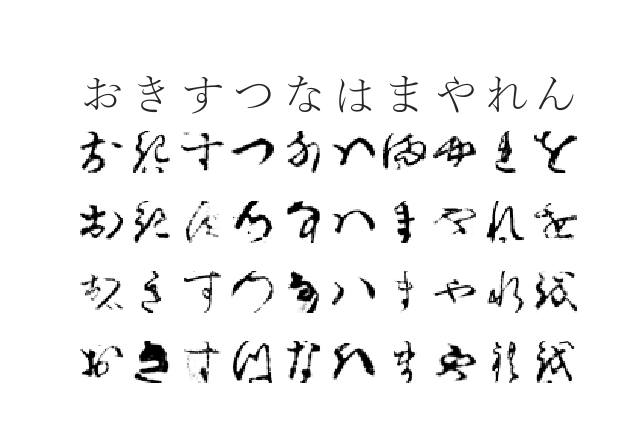
\includegraphics[width=0.6\textwidth, center]{kmnist_examples}
            \caption{Examples of images belonging to each of the 10 classes of the KMNIST dataset. The top row contains the modern-day Japanese \textit{hiragana} character, typeset, which each class represents.}
        \end{figure}
        
        
        The training dataset is provided as a 3-dimensional array of size 60000x28x28, and therefore a small amount of data preprocessing was required to "unroll" each of the 60000 observations into a one-dimensional vector of length 784. The dataset was then split by assigning each observation at random into one of three groups making up 60\%, 20\% and 20\% of the original dataset: the largest set was used for training, and the other two for hyperparameter tuning via holdout cross-validation and for final performance testing respectively. In each dataset, each input was independently rescaled on a range of 0 to 1 - not \textit{strictly} necessary in the case of this problem, since all values lay somewhere in this range anyway.
        
        Generally when deciding on a network architecture, it is useful to follow the principle of Occam's razor: in general we ought to choose the simplest model which explains the data sufficiently well. Therefore a relatively small model was defined at first, with a single hidden layer containing a few tens of neurons.
        
        However, it soon became apparent that this model was plateauing at a performance of approximately 87\% validation accuracy, even when the size of the hidden layer was increased to several hundred neurons in size.
        
        Therefore a second, smaller, hidden layer was added in an attempt to take advantage of higher-level patterns which might be present in the dataset - in practical terms, a single line of code was added defining the new layer. After some experimentation and adjustment of hyperparameters, a network with two hidden layers containing 200 and 30 neurons respectively was capable of consistently achieving approximately 93\% validation set accuracy (and 92\% test set accuracy). Figure \ref{fig:kmnist_confusion} shows examples from the test dataset which were correctly and incorrectly classified by this model, and gives some idea of the complexity of the task at hand.
        
        
        \begin{figure}[h] \label{fig:kmnist_confusion}
            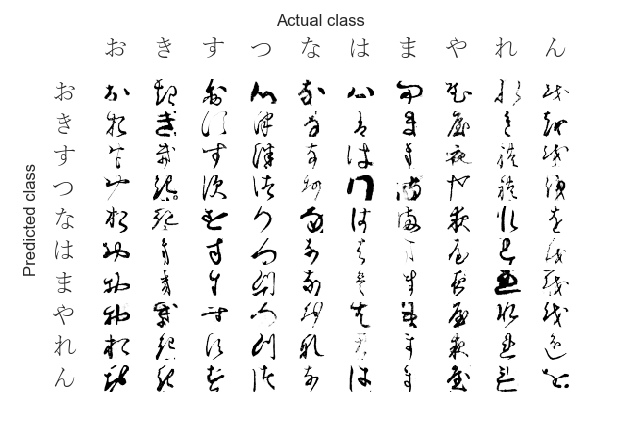
\includegraphics[width=0.8\textwidth, center]{kmnist_confusion}
            \caption{"Confusion plot" showing examples from the test dataset which were correctly and incorrectly classified by the trained two-hidden-layer model.}
        \end{figure}
        



\section{Areas for Further Work}



\bibliography{report}
\bibliographystyle{abbrv}

\end{document}
	